\section{Backgrounds}
\label{sec:od_analysis_backgrounds}

\par
Using the aforementioned energy scale and noise cut, in this section the background rate in the OD is measured and attempts are made to understand what is seen.
\par
In \autoref{fig:od_random_trigger} a comparison between the observed events in the OD during SR1 and those expected are shown.
The expected rates here are from "full-chain" simulations described in XXX, which include energy deposits, light propagation to PMTs and an electronic response.
Both data and simulations were handled by the same analysis tools.
In the simulation no PMT effects were turned on such as after pulsing and dark counts and the "noise-cut" is expected to remove those events.
\par
Neither the improved GdLS purification or the LS screener measured radioactivity are in good agreement, with a notable peak in seen in data that isn't accounted.
At the low energy, the observed rate is also higher than that expected.
In part this could be accounted for by the lower light collection efficiency, causing the observed rate to be significantly lower than expected, as discussed in Section XXX.

\begin{figure}[]
    \centering
    \begin{tikzpicture}
    
    \begin{axis}[
        xlabel=Pulse Area,
        ylabel=Rate (Hz/5phe),
        width=15cm, height=10cm,
        xmin=0, xmax=1000,
        %ymax=1e-7, 
        ymode=log,
        legend pos=north east,
        grid=major]
            
        \addplot[only marks, mark size=0.5pt,
                 error bar legend,] 
            plot[error bars/.cd, x dir=both, x explicit]
            table[x=pulsearea,y=weight,x error=xerror, y error=yerror]
            {Data/OD_Backgrounds/background_constraints/od_data.dat};
        
        \addplot[red, const plot]
            table [x=pulsearea,y=weight]
            {Data/OD_Backgrounds/background_fit/starting_point/backgrounds_improved_purification.dat};
            
        \addplot[green, const plot]
            table [x=pulsearea,y=weight]
            {Data/OD_Backgrounds/background_fit/starting_point/backgrounds_original_purification.dat};
        
        \legend{Data, Original purification, Improved purification};
        \end{axis}
    \end{tikzpicture}
    \caption{OD pulse area spectrum from using the Random Trigger in the region. 
    Only the noise cut has been applied to the data.
    Overlaid are the expected rates from all backgrounds with the improved and original GdLS internal rates.}
    \label{fig:od_random_trigger}
\end{figure}

\par
In the remainder of this section, the stability of these backgrounds and the contributions are examined.

\subsection{Rate Stability}

\par
The events in the OD were observed for a number of months, the result of which is shown in \autoref{fig:OD_SR1_Rate} along with the date range used for SR1.
The gaps in the data correspond to calibration campaigns, where a different Trigger configuration was used and the rate observed would not be representative of the true background rate so had been excluded.
\par
The various fluctuations in the noise-cut has been linked to the chiller system being turned on, indicating a grounding failure for which the noise-cut was designed.
Importantly, over this period the OD rate remains stable, with no features in the observed distribution changing during that time.

\begin{figure}[!htbp]
    \centering
   \begin{tikzpicture}
        \begin{axis}[
        date coordinates in=x,
        %xtick=data,
        xticklabel style=
        {rotate=90,anchor=near xticklabel},
        xticklabel=\day.\month.\year,
        xlabel={Date},
        %ymin=247, ymax=250,
        y tick label style={/pgf/number format/1000 sep=},
        extra y tick style={grid=major, tick label style={xshift=-1cm}},
        ylabel={Rate (Hz)},
        date ZERO=2009-08-18,% <- improves precision!
        width=15cm,
        height=6cm,
        ]
        \addplot[smooth, error bar legend,
                 error bars/.cd,
                 y dir=both, y explicit, error bar style={color=orange}] table[x=date,y=noise, y error=noise_error] {Data/OD_Backgrounds/background_rates/random_trig_rates.txt};
                 
        \addplot[smooth, error bar legend,
                 error bars/.cd,
                 y dir=both, y explicit, error bar style={color=orange}] table[x=date,y=100kev, y error=200kev_error] {Data/OD_Backgrounds/background_rates/random_trig_rates.txt};
        
        \addplot[smooth, error bar legend,
                 error bars/.cd,
                 y dir=both, y explicit, error bar style={color=orange}] table[x=date,y=200kev, y error=200kev_error] {Data/OD_Backgrounds/background_rates/random_trig_rates.txt};
                 
        \end{axis}
    \end{tikzpicture}
    \caption{Rate in OD during and before SR1 data taking on a week-by-week basis using the Random Trigger.
    Week -1 corresponds to the month prior to SR1 when the OD PMT gains were higher.}
    \label{fig:OD_SR1_Rate_spare}
\end{figure}
%\par


\begin{figure}[!htbp]
    \centering
    \begin{tikzpicture}
        \begin{axis}[
            title=TODO: Replace with dates and errors,
            xlabel=Data taking week,
            ylabel=Rate (Hz),
            width=15cm,
            height=6cm,
            xmin=-2,
            xmax=14,
            legend style = {column sep = 10pt, legend columns = -1,}]
            \addplot[red, only marks]
                    table [x=Week,y=Rate]
                    {Data/OD_Backgrounds/background_rates/od_sr1_rate_noise.dat};
            \addlegendentry{Noise Cut};
            \addplot[blue, only marks]
                    table [x=Week,y=Rate]
                    {Data/OD_Backgrounds/background_rates/od_sr1_rate_100.dat};
            \addlegendentry{100keV};
            \addplot[green, only marks]
                    table [x=Week,y=Rate]
                    {Data/OD_Backgrounds/background_rates/od_sr1_rate_200.dat};
            \addlegendentry{200keV};
        \end{axis}
    \end{tikzpicture}
    \caption{Rate in OD during and before SR1 data taking on a week-by-week basis using the Random Trigger.
    Week -1 corresponds to the month prior to SR1 when the OD PMT gains were higher.}
    \label{fig:OD_SR1_Rate}
\end{figure}

\par
During the SR1 data taking period, the rate-per-phe is shown in \autoref{fig:od_sr1_rate_vs_threshold}.
Overlaid is the expected rate of backgrounds from \autoref{tab:od_expected_rates}.
Interestingly the observed rate is below what was anticipated from energy deposit simulations.
This unexpected result means that the veto threshold could be reduced to 100keV, which should increase the veto tagging efficiency.
Alternatively, the threshold could be left at 200keV, but the window extended to 1200$\mu$s with a 5\% impact on live time.
Either way there is no concern about the requirement to limit the livetime impact not being met.

\begin{figure}[]
    \centering
    \begin{tikzpicture}
        \begin{axis}[
            xlabel=OD Threshold (phd),
            ylabel=Rate (Hz),
            width=15cm, height=8cm,
            xmin=-1, xmax=55,
            ymin=0, ymax=350,
            legend pos=north east,
            grid=major]
             \addplot+[black, smooth, mark=none]
                    table [x=Threshold,y=Rate]
                    {Data/OD_Backgrounds/background_rates/od_sr1_rate_vs_threshold_smooth_line.dat};
            \addplot[black, only marks, 
                     error bar legend,
                     error bars/.cd,
                     x dir=both, x explicit, error bar style={color=black}]
                    table [x=Threshold,y=Rate, x error=XError]
                    {Data/OD_Backgrounds/background_rates/od_sr1_rate_vs_threshold_error_bars.dat};
             \addplot[dashed, mark=none, red] coordinates {(0,100) (60,100)};
             \addplot[dashed, mark=none, blue] coordinates {(17.6,0) (17.6,350)};
             \addplot[dashed, mark=none, green] coordinates {(37.5,0) (37.5,350)};
             
             \addplot[orange, only marks, 
                      error bar legend,
                      error bars/.cd,
                      y dir=both, y explicit, error bar style={color=orange}]
                      table [x=Threshold,y=Rate, y error=YError]
                      {Data/OD_Backgrounds/background_rates/od_sr1_rate_expected.dat};
             
             \legend{,SR1 Data,$<$100Hz Requirement,100 keV (17.6 phd),200 keV (37.5 phd),Expected}                
        \end{axis}
    \end{tikzpicture}
    \caption{Rate of OD backgrounds during SR1 using the Random Trigger. The noise cut has been applied. 100Hz Requirement is for a 500$\mu$s veto window as proposed in \cite{LZ_TechnicalDesignReview_ref}. Expected values are from \autoref{tab:od_expected_rates}}
    \label{fig:od_sr1_rate_vs_threshold}
\end{figure}

%%%%%%%%%%%%
\subsection{Position Reconstruction}
\par
For any pulse it is possible to reconstruct the location of the interaction that caused the pulse by a weighted average.
This was performed using a simple weighted distribution (\autoref{eq:OD_xy_position});

\begin{equation}
    x = \frac{\sum{\text{Ch}_{\text{phe}} * \text{Ch}_\text{x}}}{\sum{\text{Ch}_\text{phe}}} 
\label{eq:OD_xy_position}
\end{equation}
Due to limited pre-SR1 calibrations, an insufficient variety of calibration sources were used at varying x-y-z positions in order to adequately determine the resolution of this approach, but it is something a future calibration campaign may be able to tackle. 
Additionally, this approach does not take into account the OCV in the centre of the detector, so reconstructed pulses will have an incorrect position, but the correct shape.
However, this provides an insight not-thought possible based upon optical simulations.
It is also possible to reconstruct the pulse $\theta$ position in a similar fashion.


\begin{figure}[!htbp]%
\centering
\begin{tikzpicture}
\centering
  \begin{groupplot}[%view={0}{90},
    group style = {group size = 2 by 3,vertical sep=3cm,
                   horizontal sep=1.5cm},
                   height=6cm, width=0.5\textwidth]
    \nextgroupplot[
            ylabel=Rate (Hz),
            xlabel=Pulse Area (phd),
            width=0.95\textwidth,
            height=6cm,
            %xshift=0.5\textwidth,
            xmin=0, xmax=800,
            ymin=1e-4, ymax=1e3,
            ymode=log,
            ]
            \addplot[only marks, mark size=1.0pt] 
            plot[error bars/.cd, x dir=both, x explicit]
            table[x=pulsearea,y=weight,x error=xerror, y error=yerror]
            {Data/OD_Backgrounds/background_constraints/od_data.dat};
            
            \addplot[dashed, mark=none, name path=A,blue] coordinates {(75,0.00001) (75,10000)};
            \addplot[dashed, mark=none, name path=B,blue] coordinates {(125,0.00001) (125,10000)};
            \addplot[dashed, mark=none, name path=C,green] coordinates {(500,0.00001) (500,10000)};
            \addplot[dashed, mark=none, name path=D,green] coordinates {(1000,0.00001) (1000,10000)};

            \addplot[blue!50] fill between[of=A and B];
            \addplot[green!50] fill between[of=C and D];
            
    \nextgroupplot[group/empty plot]

    \nextgroupplot[colorbar, 
    colorbar style={title=Rate (Hz),ymode=log,},
    width=0.4\textwidth, view={0}{90},
    xshift=-0.3\textwidth,
    ylabel=Z (cm),
	xlabel=R (cm),
	y label style={at={(axis description cs:-0.13,0.5)},anchor=near ticklabel},]
    \addplot3[
		surf,
		shader=flat corner,
		mesh/cols=50,
		mesh/ordering=rowwise,
		point meta = {z>1 ? nan : z}
		] file {Data/playground/alpha_peak_r_z.csv};
	\node [rotate=90] at (axis cs:0,1050) {Region 1};
	\nextgroupplot[colorbar, 
	colorbar style={title=Rate (Hz),ymode=log,},
	width=0.4\textwidth, view={0}{90},
    xshift=-0.5\textwidth, %yshift=1.5cm,
    ylabel=Y (cm),
	xlabel=X (cm),
	y label style={at={(axis description cs:-0.13,0.5)},anchor=near ticklabel},]
    \addplot3[
		surf,
		shader=flat corner,
		mesh/cols=54,
		mesh/ordering=rowwise,
		point meta = {z>1 ? nan : z}
		] file {Data/playground/alpha_peak_x_y.csv};

    \nextgroupplot[colorbar, 
    colorbar style={title=Rate (Hz),ymode=log,},
    width=0.4\textwidth, view={0}{90},
    ylabel=Z (cm),
	xlabel=R (cm),
	y label style={at={(axis description cs:-0.13,0.5)},anchor=near ticklabel},]
    \addplot3[
		surf,
		shader=flat corner,
		mesh/cols=50,
		mesh/ordering=rowwise,
		point meta = {z>1 ? nan : z}
		] file {Data/playground/rg_th232_r_z.csv};
		
	\nextgroupplot[colorbar, 
	colorbar style={title=Rate (Hz),ymode=log,},
	width=0.4\textwidth, view={0}{90},
	ylabel=Y (cm),
	xlabel=X (cm),
    y label style={at={(axis description cs:-0.13,0.5)},anchor=near ticklabel},]
    \addplot3[
		surf,
		shader=flat corner,
		mesh/cols=54,
		mesh/ordering=rowwise,
		point meta = {z>1 ? nan : z}
		] file {Data/playground/rg_th232_x_y.csv};
   
  \end{groupplot}
  
  \node at ($(group c1r2) + (-1.0cm, 3.5cm)$) {\textbf{Region 1 (blue)}};
  \node at ($(group c1r3) + (-1.0cm, 3.5cm)$) {\textbf{Region 2 (green)}};
  
\end{tikzpicture}
\caption{Position Reconstruction of pulses from various regions in pulse area space defined in the top plot. 
         Each pulse has had the noise cut applied and the position reconstructed using \autoref{eq:OD_xy_position}.}
\label{fig:od_backgrounds_position_reconstruction}
\end{figure}

\par
The positions of pulses in two regions of interest are shown in \autoref{fig:od_backgrounds_position_reconstruction}.
Region 1 focuses on the peak at 100phd (XXX keV).
Region 2 is in an area above 2MeV where Cavern-$\gamma$'s should dominate.
In terms of the shape distribution, there are two noticeable features in \autoref{fig:od_backgrounds_position_reconstruction}, firstly at both energy regions reconstructed, a majority of events occur in the top and bottom of the OD. 
Secondly, in (+x,+y) there is a higher rate than in the other tanks.
By labelling the SATs with letters A-D starting from (+x,+y) and going around clockwise, it is possible to understand this difference.
Using this labelling, over the period of SR1, SAT A has a rate in excess of 8\% higher than any of the other tanks, with SAT B seeing the next highest rate (3\% higher than the mean).
Both SATs C and D saw an equivalent rate.
In \autoref{fig:OD_conduit_geometry}, the SAT placement are shown along with the conduits.
SAT A and SAT B are the only tanks which are obstructed by a single conduit, additionally both tanks cover an entire BAT and TAT.
The CSD-ports and the OCV legs block the other SATs from the TATs and BATs.
This results in the light having a more direct path to more PMTs, increasing light collection.
These two effects combined can explain the increase in rate seen in SAT A and B.

\begin{figure}[!htbp]
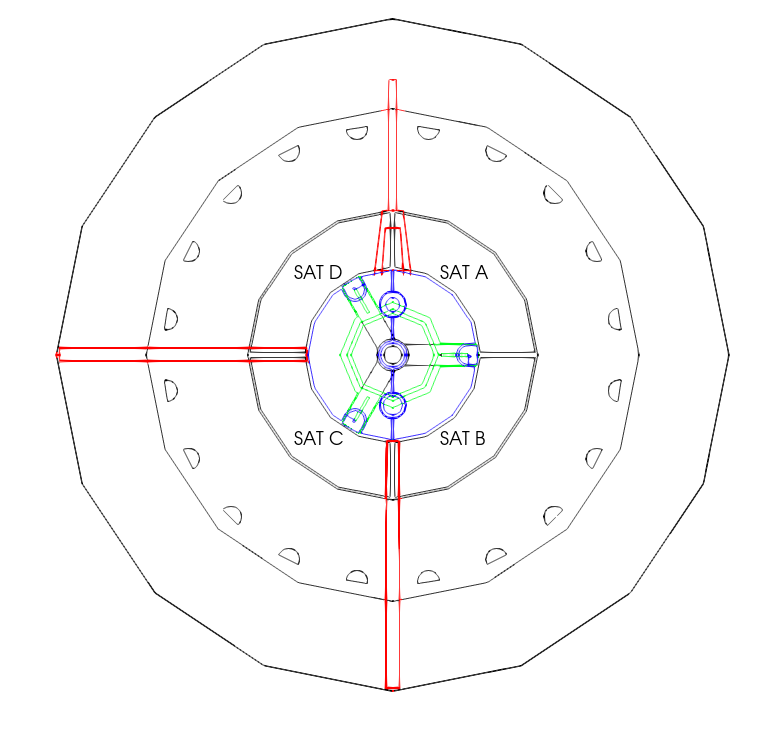
\includegraphics[width=\textwidth]{Figures/Geometry/geometry_with_conduits.png}
\centering
\caption{LZ geometry schematic. The OD geometry excluding the BATs and TATs is shown in black. The BATs and bottom on OCV are shown in green. The TATs, CSD ports and PMT conduits in blue. The DD calibration conduits and the High-Voltage feed through for the TPC are shown in red.}
\label{fig:OD_conduit_geometry}
\end{figure}

\par
The events reconstructed at the top and bottom of the OD dominate everything.
This supports both \autoref{tab:od_expected_rates} and \autoref{fig:OD_estimated_background_rate} (see \autoref{sec:simulated_od_requirements}), where cavern-$\gamma$'s are expected to be the largest contributor with the largest contribution coming from the bottom. 

\par
As a way of suppressing cavern-$\gamma$'s, a slice of events reconstructed to be in the middle of the side tanks was taken.
The resultant pulse spectrum is shown in  \autoref{fig:od_data_pulsearea_middle_tank}.
The additional population are backgrounds from ${}^{60}Co$, predominately from the OCV.
In future it may be possible to constrain the rate of this using a volume cut, but as the z-cut used here is not accurate it is unreliable to determine how large the volume selected is.
To improve this, a calibration campaign with sources are various z-positions will be required.


\begin{figure}[!htbp]
    \centering
    \begin{tikzpicture}
    
    \begin{axis}[
        xlabel=Pulse Area,
        ylabel=Rate (Hz/5phe),
        width=15cm, height=10cm,
        xmin=0, xmax=800,
        ymin=1e-4, ymode=log,
        legend pos=north east,
        grid=major]
            
        \addplot[only marks, mark size=0.5pt] 
            plot[error bars/.cd, x dir=both, x explicit]
            table[x=pulsearea,y=rate,x error=x_error, y error=y_error]
            {Data/OD_Backgrounds/background_constraints/od_data_pulsearea_middle_tank_binwidth_5.dat};
            
        \end{axis}
    \end{tikzpicture}
    \caption{OD pulse area spectrum from pulses reconstructed to the middle of the OD side tanks, suppressing the rate from Cavern-$\gamma$'s.}
    \label{fig:od_data_pulsearea_middle_tank}
\end{figure}



\subsection{$\gamma$ constraints}
\par
Another area to look at is high energy $\gamma$'s, from ($\alpha$,$\gamma$) reactions, which were discussed in \autoref{sec:cavern_gamma_generator}.
What can be seen in \autoref{fig:od_high_energy} is that the rate of events expected is significantly greater than that observed.
The findings here support that the statistical model used does not extend well to ${}^{17}O$.
However, there are still features seen in data between 1000 and 1800 phd that are not accounted for in simulations.
These features can in fact be attributed to neutron captures on the Iron of the water tank producing high energy $\gamma$'s.
These neutrons originate primarily from the ${}^{252}Cf$ calibration source, which was stored in a movable safe underground during SR1.
It was moved during SR1 which matches with a change in the position of these high energy events being reconstructed.
Backgrounds of this type were not previously considered within LZ, though are of great importance in fusion experiments \cite{iter_neutrons_ref}.

\begin{figure}[]
    \centering
    \begin{tikzpicture}
    
    \begin{axis}[
        xlabel=Pulse Area (phd),
        ylabel=Rate (Hz),
        width=15cm, height=10cm,
        xmin=400, xmax=3000,
        %ymax=1e-7, 
        ymode=log,
        legend pos=north east,
        grid=major]
            
        \addplot[only marks, mark size=0.5pt,
                 error bar legend,] 
            plot[error bars/.cd, x dir=both, x explicit]
            table[x=pulsearea,y=weight,x error=xerror, y error=yerror]
            {Data/OD_Backgrounds/background_constraints/od_data.dat};
            
        \addplot[red, const plot]
            table [x=pulsearea,y=weight]
            {Data/OD_Backgrounds/background_fit/starting_point/backgrounds_original_purification.dat};
            
        \legend{Data, Expectation};
        \end{axis}
    \end{tikzpicture}
    \caption{OD pulse area spectrum for high energy $\gamma$ events compared to the expected rate.
             The events observed in data between 1000 and 1800 phd are high energy $\gamma$-rays from neutron capture the iron.}
    \label{fig:od_high_energy}
\end{figure}

\par
Primarily due to the source safe placement during SR1, it was not possible to ascertain if there was a fluctuation in the high-energy $\gamma$-rate during SR1.
Though in future runs this can be an area of study, similar to \cite{cavern_gamma_annual_modulation_CoGeNT_ref, cavern_gammas_in_Soudan_mine_ref}.

%%%%%%%%%%%%
\subsection{$\alpha$ constraints}
\par
Though the exact rate of GdLS is not known, it is possible to constrain some of the components observed.
Notably, decays within the U and Th decay chains where the second decay has a short enough half-life such that it is within the LZ event window.
This leaves 3-possible decays, summarised in \autoref{tab:od_constrainable_decays_in_data}.
However, in reality only  ${}^{214}Bi \to {}^{214}Po$ and ${}^{219}Rn \to {}^{215}Po$ can be searched for as the interactions from ${}^{212}Bi \to {}^{212}Po$ are close enough together that they will be merged into one pulse.

\begin{table}[!htbp]
    \centering
    \begin{tabular}{c|c|c|c|c|c}
        \multirow{2}{*}{Decay Pair (chain)}                    & \multicolumn{2}{c|}{First Decay}   & \multicolumn{3}{c}{Second Decay}    \\ 
                                                               & Decay    & Energy (MeV) & Decay    & Energy (MeV) & half-life ($\mu$s) \\ \hline
        ${}^{214}Bi \to {}^{214}Po$ (${}^{238}U_{m}$)          & $\beta$  & 3.27         & $\alpha$ & 7.83         & 160   \\ 
        ${}^{219}Rn \to {}^{215}Po$ (${}^{235}U_{l}$)          & $\alpha$ & 6.95         & $\alpha$ & 7.53         & 1800  \\ 
        ${}^{212}Bi \to {}^{212}Po$ (${}^{232}Th_{l}$)         & $\beta$  & 2.25         & $\alpha$ & 8.95         & 0.3
    \end{tabular}
    \caption{Th and U decay chain pairs with half-lives within the LZ event window of 4.5ms. See \autoref{fig:decay_chains} for the complete Decay Chains.}
    \label{tab:od_constrainable_decays_in_data}
\end{table}

\par
The decay pairs can be searched for by looking for pulses which are reconstructed to be close to each other in position.
The position requirement is to reduce the impact of coincident interactions and decays in other areas of the OD.
As the second decay is an $\alpha$ it does not have significant penetrating power so the interaction will be close to where the initial decay was.
The cut implemented loosely to account for potential variable inefficiencies in the position reconstruction with z and $\theta$.
The final selection used was a $z_{diff} < 100$ and $\theta_{diff} < 1.0$, where $diff$ refers to the difference between pulses.
The result of this is shown in \autoref{fig:od_bipo_alphas_2d}.
Only pulses above 200keV in visible energy are included.

\begin{figure}[!htbp]%
\centering
\begin{tikzpicture}
\centering
  \begin{axis}[
    height=10cm, width=10cm,
    view={0}{90},
    ylabel={Second Pulse (phd)},
    xlabel={First Pulse (phd)},
    colorbar,
    colorbar style={ylabel={Rate (Hz)},ymode=log,},
    ]
    \addplot3[
      surf,
      shader=flat corner,
	  mesh/cols=40,
	  mesh/ordering=rowwise,
	  point meta = {z<0.0000001 ? nan : z}
    ] file {Data/OD_Backgrounds/background_constraints/rnpo_rate_2d.dat};

  \end{axis}
\end{tikzpicture}
\caption{Relationship of pulses reconstructed in close proximity to each other. Only pulses above 200 keV have been included.}
\label{fig:od_all_pulse_pairs_2d}
\end{figure}

\begin{figure}[!htbp]%
\centering
\begin{tikzpicture}
\centering
  \begin{groupplot}[%view={0}{90},
    group style = {group size = 1 by 2,vertical sep=1.5cm,
                   horizontal sep=1.5cm},
                   height=6cm, width=0.5\textwidth]

	\nextgroupplot[height=10cm, width=10cm,
    view={0}{90},
    ylabel={Second Pulse (phd)},
    xlabel={First Pulse (phd)},
    colorbar,
    colorbar style={ylabel={Rate (Hz)},ymode=log,},
    ]
    \addplot3[
      surf,
      shader=flat corner,
	  mesh/cols=40,
	  mesh/ordering=rowwise,
	  point meta = {z<0.0000001 ? nan : z}
    ] file {Data/OD_Backgrounds/background_constraints/rnpo_rate_2d.dat};
    
    
    \nextgroupplot[height=10cm, width=10cm,
    view={0}{90},
    ylabel={Second Pulse (phd)},
    xlabel={First Pulse (phd)},
    colorbar,
    colorbar style={ylabel={Rate (Hz)},ymode=log,},
    ]
    \addplot3[
      surf,
      shader=flat corner,
	  mesh/cols=40,
	  mesh/ordering=rowwise,
	  point meta = {z<0.0000001 ? nan : z}
    ] file {Data/OD_Backgrounds/background_constraints/bipo_rate_2d.dat};
   
  \end{groupplot}
\end{tikzpicture}
\caption{Relationship of pulses reconstructed in close proximity to each other. Only pulses above 200 keV have been included.
         \textbf{Top:} All pulses-pairs within 800 $\mu$s of each other. The distribution is from ${}^{214}$Bi $\to {}^{214}$Po.
         \textbf{Bottom:} All pulse-pairs with more than 800 $\mu$s time separation between them. The distribution left is from ${}^{219}$Rn $\to {}^{215}$Po.
         }
\label{fig:od_time_dependent_pulses_2d}
\end{figure}



\par
The distribution around 170phd in both pulses correspond to the $\alpha$'s in the ${}^{235}U_{l}$ chain.
Although less clear, the second pulse contains a second $\alpha$ around the same place, and a $\beta$ spectrum in the first pulse.
This becomes easier to see in when the features are extracted as is shown in \autoref{od_bipo_alphas}.

\begin{figure}[!htbp]%
\centering
\begin{tikzpicture}
\centering
    \begin{axis}[
            ylabel=Rate (Hz/2keV),
            xlabel=Energy (MeV),
            width=15cm,
            height=8cm,
            grid=major,
            xmin=0, xmax=3,
            ymin=1e-4, ymode=log,]
            
        \addplot[red, only marks, mark size=1, 
                 error bars/.cd,
                 y dir=both, y explicit, error bar style={color=black}]
            table [x=energy,y=rate,y error plus index=2, y error minus index=3]
            {Data/OD_Backgrounds/background_constraints/od_bipo_first_alpha.dat};
            
        \addplot[blue, only marks, mark size=1, 
                 error bars/.cd,
                 y dir=both, y explicit, error bar style={color=black}]
            table [x=energy,y=rate,y error plus index=2, y error minus index=3]
            {Data/OD_Backgrounds/background_constraints/od_bipo_second_alpha.dat};
                
    \end{axis}
            
\end{tikzpicture}
    \caption{$\alpha$ energies in from BiPo and RnPo.}
    \label{fig:od_bipo_alphas}
\end{figure}

\par
The second pulse distribution peak is broadened due to two Gaussian's contributing to it, from two $\alpha$'s.
One from ${}^{214}Po$ and one from ${}^{215}Po$.
We are able to constrain the rate of these events by using a reverse search, finding the second $\alpha$ in the energy range and then looking for the first decay.
This gives a rate of 90mHz for ${}^{214}Bi \to {}^{214}Po$, which is within 50\% that expected from the 'improved purification' (see \autoref{sec:simulated_od_requirements}).
Measuring the rate of ${}^{219}Rn \to {}^{215}Po$ is performed in a similar way giving a rate of XXX, though with an addition time constraint accounting for several decay-constants worth of time which is lower than the decay half-life of ${}^{214}Po$.
The selection of this data is shown in \autoref{fig:od_bipo_alphas_2d_2}.
This is again within 50\% of that from the 'improved purification', and so the assumption can be made that this purification was done, and that the estimated rates can be assumed true for all decays.


\par
Importantly, these constraints indicate that the $\alpha$-peak seen in \autoref{fig:od_random_trigger} is not from those subchains, as the rate would be too low.
This opens up the possibility that it is from ${}^{210}Po$ from the late chain of ${}^{238}U$.
This claim appears at odds with the relatively low internal rate of ${}^{238}U$.
However, it is known and measured that there is significant $Rn$ in the cavern air, and as previously discussed (\autoref{sec:od_construction_sec}) the acrylic tanks were open to the air for long periods prior to installation.
There was opportunity for decay daughters to plate-out on the inside of the acrylic tanks, a feature that is of great concern within the TPC \cite{radon_plateout_ref}.
${}^{210}Pb$ is the only long-lived particle in the Radon chain, with a half-life in excess of 22-years. 
The remainder of the isotopes would drastically reduce in abundance after a few weeks, leaving only ${}^{210}Pb$ daughters visible, at a sustained rate.
This allows the acrylic holding the scintillator to act as a reservoir, providing a constant supply of $\alpha$ decays from ${}^{210}Po$.
LZ is not alone in having experienced this, with KamLAND measuring a higher than expected rate of ${}^{238}U_l$ decays \cite{KamLAND_LS_contaminants_ref}.

\par
Although it is unexpected to see a four $\alpha$'s, it becomes possible to perform an $\alpha$ energy calibration, and will be continuously measurable during all Science runs, without the need for Science data taking to be stopped.
An additional advantage is that PMT gain-drift will be more easily detectable.
The observed energy of each of the $\alpha$'s verse the observed energy are shown in \autoref{fig:od_alpha_quenching}, the Birk's law fit is also provided using the parameters in \autoref{tab:Birks_law_parameters}.
It can be seen that the parameters taken from pure LAB remain in good agreement with Gd-doped LAB used here.
This also isolates the difference between observed data and simulations to light propagation.

\begin{figure}[!htbp]%
\centering
\begin{tikzpicture}
\centering
    \begin{axis}[
            ylabel=Visible Energy (MeV),
            xlabel=Particle Energy (MeV),
            width=15cm,
            height=8cm,
            grid=major,
            xmin=0, xmax=10,
            ymin=0,
            legend pos=north west,
            ]
            
        % Birks Fit
        \addplot[red]
            table [x=Energy,y=Quenched]
            {Data/GdLS_Physics/Quenching/alpha.dat};
        \addplot[black, only marks, mark size=1, 
                 error bars/.cd, error bar style={color=black},
                 y dir=both, y explicit,]
            table [x=energy,y=observed,y error plus index=2, y error minus index=3]
            {Data/OD_Backgrounds/background_constraints/od_alpha_energies.dat};
        \legend{Birk's, Measured};
    \end{axis}
            
\end{tikzpicture}
    \caption{Observed energy vs particle energy from $\alpha$ particles.
             The expected quenching from Birk's Law using the parameters in \autoref{tab:Birks_law_parameters} is shown to be in good agreement with what is observed.}
    \label{fig:od_alpha_quenching}
\end{figure}

\subsection{${}^{152}Gd$}
\par
The final background that can be constrained is ${}^{152}Gd$, which produces a 2.2MeV $\alpha$ decay.
Though this is of particular use as can be seen in Figure XXX where ${}^{14}C$, ${}^{152}Sm$ and ${}^{152}Gd$ all can contribute to that region.
The GdLS is loaded with 0.1\% (by mass) of natural Gadolinium.
With a total mass of GdLS used in the detector this corresponds to 16000kg, and ${}^{152}Gd$ has a natural abundance of 0.2\%, this gives a maximum possible rate of 27Hz, where there is a 5\% uncertainty on the doping by mass.

\subsection{Background Fitting}
\par
Given the constraints placed on rates, it is possible to fit the expected distribution to data. 
The fit was limited to only include the region of the simulation which is approximately correct with the data. 
As such, the high energy, above 500phd ($\gtrsim$ 2.5MeV) was excluded, and a low energy cut was 20phd was used.
\par
In order to keep the number of fit parameters down, all detector components were in combined.
Given the mitigation procedure described in \autoref{sec:od_construction_sec}, the contamination is likely to be minimal from these components.
\par
Another source, ${}^{7}Be$, which has been considered in fits from similar experiments has been excluded here.
As it only has a half-life of 50-days (TODO CITE XXX), and the OD was not in a stable running condition until nearly a year after filling, it has been assumed that the contribution from ${}^{7}Be$ would be negligible.
\par
For fitting the background, this leaves a total of XXX components.
The cavern-$\gamma$'s were allowed to float within the uncertainties they were measured in \cite{LZ_Gamma_Ray_Background_ref}.
The ${}^{235}U_e$, ${}^{235}U_l$, ${}^{238}U_e$, ${}^{238}U_m$, ${}^{238}U_l$, ${}^{232}Th_e$, ${}^{232}Th_l$ where constrained to be in equilibrium with the sub-chains, and constrained by the LS Screener result or the measured $\alpha$-rate here, with the exception of ${}^{238}U_l$ which was able to float freely.
The internal decays were left to float as freely as possible.



\begin{table}[!htbp]
    \centering
    \begin{tabular}{c|c|c|c}
        Source              &  Decay Type(s)             & Estimated Rate (Hz)       & Measured Rate (Hz) \\ \hline
        ${}^{238}U_{e}$     & $\gamma$,$\alpha$,$\beta$  & 3.27                      &                     \\ 
        ${}^{238}U_{m}$     & $\gamma$,$\alpha$,$\beta$  & 3.27                      &                     \\
        ${}^{238}U_{l}$     & $\gamma$,$\alpha$,$\beta$  & 3.27                      &                     \\
        ${}^{235}U_{e}$     & $\gamma$,$\alpha$,$\beta$  & 3.27                      &                     \\
        ${}^{235}U_{l}$     & $\gamma$,$\alpha$,$\beta$  & 3.27                      &                     \\
        ${}^{232}Th_{e}$    & $\gamma$,$\alpha$,$\beta$  & 3.27                      &                     \\
        ${}^{232}Th_{l}$    & $\gamma$,$\alpha$,$\beta$  & 3.27                      &                     \\
        Detector Components & $\gamma$,$\beta$           & 3.27                      &                     \\
        ${}^{40}K$          & $\gamma$,$\beta$           & 3.27                      &                     \\
        ${}^{85}Kr$         & $\gamma$,$\beta$           & 3.27                      &                     \\
        ${}^{14}C$          & $\beta$                    & 3.27                      &                     \\
        ${}^{176}Lu$        & $\gamma$,$\beta$           & 3.27                      &                     \\
        ${}^{147}Sm$        & $\alpha$                   & 3.27                      &                     \\
        ${}^{152}Gd$        & $\alpha$                   & 3.27                      &                     
        
        
    \end{tabular}
    \caption{Th and U decay chain pairs with half-lives within the LZ event window of 4.5ms. See \autoref{fig:decay_chains} for the complete Decay Chains.}
    \label{tab:od_constrainable_decays_in_data}
\end{table}